\documentclass[11pt,a4paper]{article}

\usepackage{graphicx}
\usepackage{sidecap}
\usepackage{mathtools}
%Om grotere integralen te krijgen
\usepackage{relsize}

%Andere breedte en lengthe van een document
\setlength{\textwidth}{6in} 
\addtolength{\hoffset}{-0.5in}
\setlength{\topmargin}{-0.2in}
\setlength{\textheight}{9in}

%Packages voor de figuren:
\usepackage{wrapfig}
\usepackage{caption}
\usepackage{subcaption}
%Kan er voor zorgen dat een figuur op de exacte plaats staat:
\usepackage{float}

\begin{document}
\title{\Huge Numerieke Wiskunde}
\author{Joni Allaert\\
		Ward Schodts\\
		}

\date{2013 - 2014}
\maketitle
\thispagestyle{empty}

\newcount\mycount
\begin{center}


\includegraphics[scale=0.4]{KULzwart.png}

\end{center}
\begin{center}
\Large Professor Dr. ir. Marc Van Barel
\vfill
\end{center}
\titlepage
\section{Deel 1: numerieke integratie}
\subsection{Vast Deelinterval}
\subsubsection*{(a) Benadering van de integralen $\mathop{\mathlarger{\int\limits_{-1}^1e^xdx}}$ en  $\mathop{\mathlarger{\int\limits_{-5}^5\frac{1}{1+x^2}}}$}

\begin{figure}[H]

	\begin{subfigure}{0.5\textwidth}
	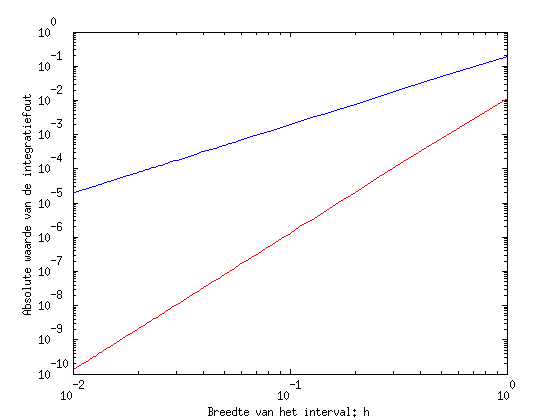
\includegraphics[width=\textwidth]{11a1.png}
	\caption*{$\int\limits_{-1}^1e^xdx$ met de trapeziumbenadering in het blauw en met de simpsonbenadering in het rood.}
	\end{subfigure}
	%Laat hier geen lijnen tussen anders komen ze niet meer horizontaal gelijk
	\begin{subfigure}{0.5\textwidth}
	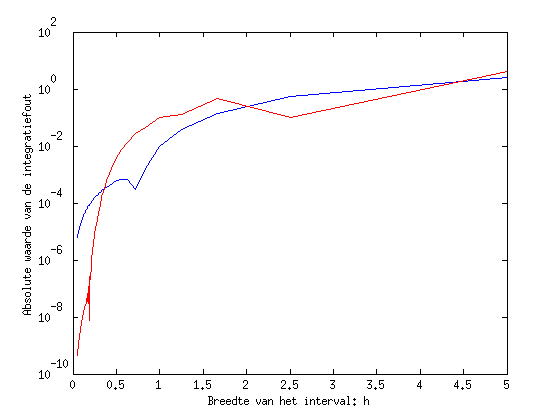
\includegraphics[width=\textwidth]{11a2.png}
	\caption*{$\int\limits_{-5}^5\frac{1}{1+x^2}$ met de trapeziumbenadering in het blauw en met de simpsonbenadering in het rood.}
	\end{subfigure}

\end{figure}


\end{document}